\documentclass[12pt,a4paper]{article}
\usepackage{listings}
\usepackage{graphicx}
\usepackage{epstopdf}
\usepackage{url}
\usepackage{amsmath,amsfonts,amssymb,amsthm}
\usepackage{caption}
\usepackage[a4paper,inner=3cm,outer=3cm,top=2cm,bottom=3cm]{geometry}
\newcommand{\func}[1]{{\bfseries \slshape \nobreakdash #1}}
\newcommand{\keyword}[1]{{\bfseries \nobreakdash #1}}
\lstset{
breaklines=true,
frame=single,
keepspaces=true,
captionpos=b
}

\tolerance 1414
\hbadness 1414
\emergencystretch 1.5em
\hfuzz 0.3pt
\widowpenalty=10000
\vfuzz \hfuzz
\raggedbottom

\begin{document}
\title{Implementing and Optimizing Washall's Algorithm using CUDA}
\author{Zhao Tuowen\\
StdID:5110309458
}
\maketitle
\begin{abstract}

This the experiments report for the course of High Performance Computing. The main purpose is to realize \keyword{Washall's Algorithm} under the \keyword{GPU Architecture} using \keyword{CUDA}, and to optimize the implementation, as well as compare the execution time of different approaches, which also includes a sequential program running on the CPU. In the end of this report also provide some thoughts gathered through this experiment on how to effectively enhance the performance of a CUDA program.

\end{abstract}

\section{Introduction}

\keyword{Washall's Algorithm}, also known as the \keyword{Floyd-Washall's Algortims}, \keyword{Floyd's algorithm}, \keyword{Roy–Warshall algorithm}, \keyword{Roy–Floyd algorithm}, or the \keyword{WFI algorithm}, is a fast method to compute the minimum distance between any two arbitrary vertices, and can also compute the transitive closure of a given graph. 

The idea behind the \keyword{Washall's Algorithm} is dynamic programming: if the minimal distance between any two vertices is known with the path only consist of a subset of the vertices, $V'$ , then we can add a new vertex $v$, and obtain the minimal distance with path containing the vertices in $V'+v$, by "relaxing" the distance of paths between all pairs of $ x,y \in V' $ with the newly added vertex $v$ through this formula, $ d_{xy} = \min{\{d_{xv}+d_{vy},d_{xy}\}} $.

By closely analyze the algorithm, we find that the correctness of it holds as long as there doesn't exist an negative circle, that is, for every $ v \in V $, $d_{vv}^{min} \geq 0$.

\lstinputlisting[language=VHDL,caption=Pseudo-code for the Basic Washall's Algorithm]{washall}

Notice that the ordering of the (i,j) pair is inconsequential. In a single iteration of k, $d_{ij}$ is only dependent on $d_{ik}$ and $d_{kj}$; $d_{ik}$,$d_{kj}$ are independent:

We can assume that $d_{ik}^{new}$ is dependent on some value, and prove it by contradiction. Then we have $d_{ik}^{old} < d_{ik}^{old}+d_{kk}$. Then we must have $d_{kk}<0$ which contradicts with the assumption that the graph contains no negative circle. Thus proved.

\subsection{The GPU Architecture}

Originally designed for computer graphics, the GPU follows a different line of evolution from CPU. The graphics processor was designed to work at the pixel level; massive parallelism is adopted to provide more processing power. 

I used Nvidia 770 GTX during the programming and testing phase of this experiments. This graphics card has 1536 CUDA cores, with memory bandwidth 224.3 GB/sec, and support compute capability 3.0 \cite{GTX770}.

At hardware level, the device consist of 8 \keyword{SIMD Multiprocessors} , \keyword{SM} ; each multiprocessor contains 196 CUDA cores and can to compute the same instruction on multiple data, hence SIMD. The execution is synchronized by warps; each warp consists of 32 different execution threads. Some of it can be masked to execute nothing if the threads diverge\cite{CBEST}. 

Each SM have constant \& texture caches, and a shared memory block. Every thread registered to the same SM can access the shared memory, acting like cache in the CPU, a staging area for the data in the global memory space. However, in CUDA, the shared memory is managed explicitly. Namely, it is manipulated using specific instruction for loading and storing. Also, it is mapped into 16 different banks to improve access speed for multidimensional data. A store/load can be completed in a single instruction if the threads in a half-warp access elements in different banks or the same one\cite{CUDAC}.

At software level, The threads are specified by \keyword{kernels} in the source, and are mapped to a maximum two three-dimensional space. The first three-dimensional space is the blocks. Each block is accessed through \func{threadIdx} and \func{blockDim} in the kernel. The second three-dimensional space is the grids. Each grid is accessed through \func{blockIdx} and \func{gridDim} in the kernel.The host can invoke a kernel using this piece of code\cite{CUDAC}:
\begin{lstlisting}[frame=none,language=C]
KernelName<<<GridDimension,BlockDimension>>>
	( ... Params ... );
\end{lstlisting}



\subsubsection{Naive CUDA Implementation}

This implementation is the most straight forward way. Every time invoke the kernel that compute all $d_{ij}$ for a specific k, as shown in the pseudo-code. The value of k is enumerated in a loop in the host code.

\lstinputlisting[language=C++,caption=Host Code for Naive Washall's Algorithms]{host}

\lstinputlisting[language=C++,caption=Kernel Definition for Naive Washall's Algorithms]{device}

This program creates a thread for every element to be updated; every block is bounded by the number of threads it can hold; the map is padded so that no divergence of control flow is needed. The thread per block number is fixed at 256 to keep the kernel occupancy high.

\subsubsection{Reusing Data}

This implementation is a slightly improved one of the previous version, in that every thread computes multiple elements instead of one, marginally reduced the total reads from the global memory. Each threads access elements in strides so that the read and write from the global memory space is coalesced:The m\textsuperscript{th} element thread accesses is with index start+i+m*stride. Each thread in this implementation compute 4 elements.

\subsection{Result and Comparison}

These two kernels are memory intensive in that they only perform limited operation on every elements to be transmitted through the bandwidth. As pictured in the following graph, the second is not much better than the first in that the data reuse is limited: every elements had to read and write at least once for each value of k to do the comparison.
\begin{figure}[ht]
\centering
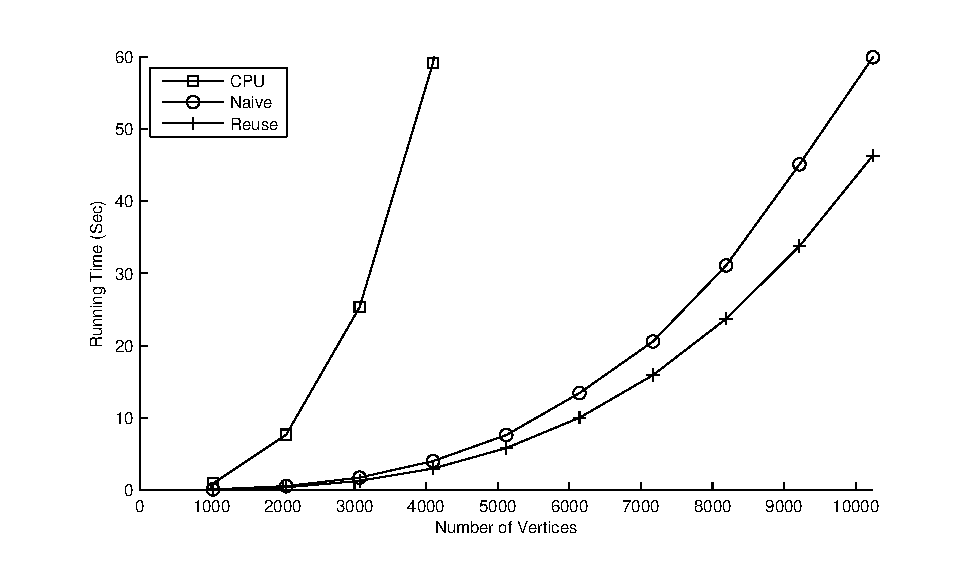
\includegraphics[
width=12cm]{cnr.eps}
\caption{Comparison between CPU, Naive CUDA, and CUDA with Reusing}
\end{figure}

Both of the CUDA version achieves 100\% occupancy, but the performance is reduced by insufficient use of global bandwidth and the extremely imbalanced use of function unit. For a element to be updated, 3 reads and a write though the global memory bus is executed, but only compute one addition and a compare. The second version improved but a little: only 3/4 read is reduced from the equation. 

Due to the memory intensive nature of this algorithm. We can use the following formula to measure the bandwidth usage in order to quickly compare different method(the lower the better):
\[ \mu = \frac{Number\:of\:read\:\&\:write}{Block\:width \footnotemark[1] } \]
\footnotetext[1]{The block width is 1 in these two programs.}
When the memory bandwidth is the most influential problem, the speed-up can be roughly calculated as:
\[ Speed Up = \frac{\mu_{old}}{\mu_{new}} \]

The speed up of the second version of the CUDA program is estimated as 1.200. Using the execution time obtained with 11264 vertices, the actual speed up is 1.282. The estimation is not far off from the real one.

\section{Blocked Approach}

Han et al.\cite{Han06} suggested the blocked approach to allow loop unrolling and cache utilization under the CPU architecture. However, it also greatly improve data reuse, and shared memory usage, through calculating multiple instances of k in one go.

By closely analysis the data dependency of the algorithms between different iterations of k. During several consecutive loops of k, from a to b. $I=\{ d_{ij}| i,j \in [a,b]\}$ only depends on the values in itself, which we call it the independent block. $S=\{ d_{ij}| i or j \in [a,b], but not both \}$ only depends on the values of itself and that of the independent block, which we termed the singly-dependent block. All other elements $d_{ij}$ depends on the values in $S$, which we call it the doubly-dependent block. This three set constitute all of the data elements in the graph. And we can compute according to the orders above, as shown in the following code( $N$ is divisible by $bw$, block width):

\lstinputlisting[language=VHDL,caption=Block Washall's Algorithm ]{blocked}

Lund and Smith\cite{Lun10} proposed \keyword{Staged blocked Method} to improve the performance by allowing more thread blocks resident on a SM through reducing usage of shared memory and utilizing the register space. However, for device with compute capability 3.0, this seems hardly necessary unless larger blocks($ >32 $) are used.

\subsection{Result and Comparison}

Using the formula suggested in the previous section we can estimate the expected speed up. However, the complexity of the program is to increase using the blocked method and using staged-load. The result may deviate by a constant factor when the programming technique change.

For the naive method:
\[ \mu = \frac{3+1}{1} \]

For the block method with block width 32:
\[ \mu = \frac{3+1}{32}  \]

For block width 32, the memory bandwidth is no longer the most prominent problem. However, to further reduce the problem, we can use a block width of 64, using similar tweaks in the Staged-blocked Method.
\[ \mu = \frac{3+1}{64}  \]

Also, to avoid overuse of registers causing the kernel occupancy to drop, we can add a directive to the definition\cite{CUDAC}.

\begin{lstlisting}[language=C,caption=Upper-bonding Register Usage]
__global__ void
__launch_bounds__(maxThreadsPerBlock, minBlocksPerMultiprocessor)
MyKernel(...)
{
    ...
}
\end{lstlisting}

However, this is not done by some tricky manipulation on the register itself, such as register packing to pack several short operand in a single register. Rather it is done by simply spilling that extra space needed to the local storage, which may cause some performance lost.
 
All of the program is implemented using similar coding style and all achieved 100\% kernel occupancy, theoretically. The performance of these methods is shown in the following graph.
\begin{figure}[ht]
\centering
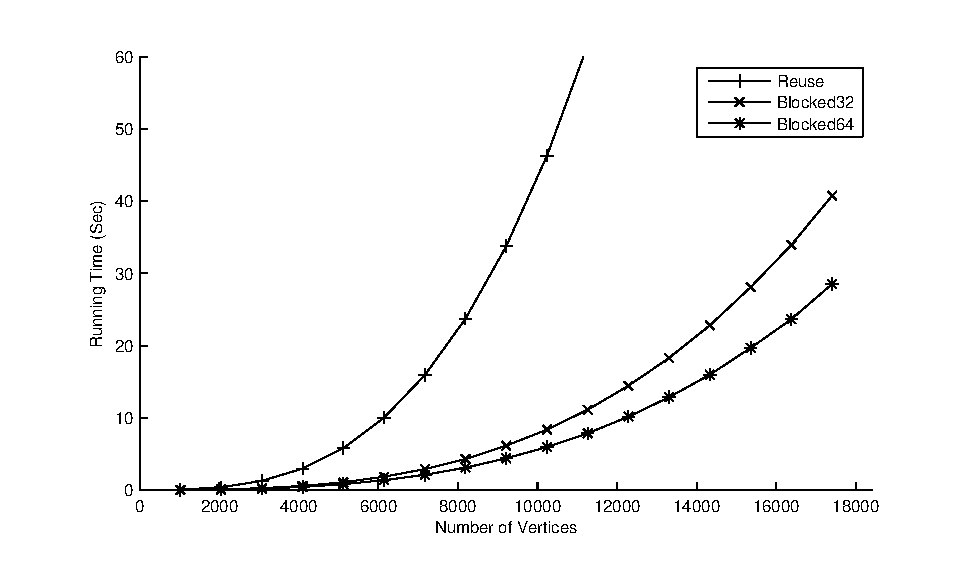
\includegraphics[
width=12cm]{rbs.eps}
\caption{Comparison between CPU, Naive CUDA, and CUDA with Reusing}
\end{figure}

The prominent kernel (for doubly-dependent blocks) in the staged-blocked method with block width of 64 achieves balanced usage of function unit and memory,  good utilization of shared memory, low local memory use, and theoretically full kernel occupancy. However, this algorithm still heavily relies on the load/store functions unit.
\begin{figure}[!ht]
\centering
\includegraphics[
width=12cm]{kernel.PNG}
\caption{ Comparison between Compute and Memory Utilization}
\end{figure}
\begin{figure}[!ht]
\centering
\includegraphics[
width=12cm]{occupancy.PNG}
\caption{ Achieved Occupany(theoretical) and Limiting Factors }
\end{figure}
\begin{figure}[!ht]
\centering
\includegraphics[
width=12cm]{compute.PNG}
\caption{ Load Comparison between Different Function Unit }
\end{figure}

\section{Conclusion}

There are several notions of great importance in improving the performance of a CUDA program. 
\begin{itemize}
  \item Kernel occupancy
  \item Control flow divergence
  \item Function unit usage
\end{itemize}

\keyword{Kernel occupancy} can hide data latency. When one warp waiting for a memory transaction, a branch jump, or a synchronization point, another can resume its execution. It is limited by the resources available under the compute capability of the device, for example:
\begin{itemize}
  \item Maximum threads per block
  \item Maximum threads per SM
  \item Maximum blocks per SM
  \item Maximum warp per SM
  \item Shared memory per SM
  \item Maximum Register per SM
\end{itemize}

\keyword{Control flow divergence} will cause threads in a warp to execute different instructions. Actually, they won't execute any differently, some threads actions are just masked by the SM, which means that their action become partly serialized. This can cause the most severe damage to the overall performance.

\keyword{Function unit usage} can improve parallelism in execution. The arithmetic unit can continue to work while a data transaction is occurring. A biased usage may cause the thread to be constantly waiting for one unit to free up, and the performance is thus limited by the throughput one type of unit.

Beyond these are more of improvements to the algorithm than that to the adaptation.

As evident in the analysis, CUDA provide an efficient way to program the GPU for general purpose calculations, which sometimes can be hundreds time faster.

However, the interface between the host and device is too complicated and exposed too much detail of the machine to the programmer. The difference between different device is huge\cite{CUDAC}. As a result, to maximize performance, optimization has to be done under every specific environment. 

The control flow is extremely simple, which on the one hand greatly simplified synchronization issues, while on the other hand hugely limited the complexity of the program. From my experience, instead of one bulky kernel to include everything, several lightweight kernels that operate in conjunction and each complete one simple step often prove to be more efficient. Also, this causes CUDA to be naturally data intensive. Complex calculations that calls for too much branching will be much less efficient.

In short, CUDA offers powerful alternative in tackling massively-parallel problems, but one has to be extra wary in designing the software to fully utilize its potential.

\bibliographystyle{abbrv}
\bibliography{hpcref}

\section*{Appendix A Program Time Chart}

\begin{table}[h]
\centering
\begin{tabular}[c]{| r || c | c | c | c | c |}
  \hline
    & \multicolumn{5}{|c|}{Execution Time (millisecond)} \\
  \hline
  Vertices & CPU & Naive & Reuse & Blocked(32) & Blocked(64)\footnotemark[1] \\
  \hline
  \hline
  1024 & 890 & 75.4846 & 48.6206 & 10.8614 & 10.5695 \\
  \hline
  2048 & 7672 & 535.468 & 374.634 & 78.0474 & 65.5086 \\
  \hline
  3072 & 25306 & 1722.28 & 1255.93 & 249.828 & 198.287 \\
  \hline
  4096 & 59118 & 3999.22 & 2971.7 & 560.264 & 429.572 \\
  \hline
  5120 & 115346 & 7620.96 & 5797.44 & 1074.35 & 802.604 \\
  \hline
  6144 &  & 13430.3 & 10012.3 & 1837.27 & 1352.21 \\
  \hline
  7168 &  & 20570.4 & 15903.4 & 2892.66 & 2103.58 \\
  \hline
  8192 &  & 31098.2 & 23721.6 & 4288.22 & 3092.14 \\
  \hline
  9216 &  & 45104.8 & 33785.8 & 6143.36 & 4384.66 \\
  \hline
  10240 &  & 59932.8 & 46330.6 & 8359.62 & 5941.12 \\
  \hline
  11264 &  & 79063.6 & 61671.4 & 11114.2 & 7856.6 \\
  \hline
  12288 &  &  &  & 14432.1 & 10162.6 \\
  \hline
  13312 &  &  &  & 18293.8 & 12847.6 \\
  \hline
  14336 &  &  &  & 22818.8 & 15987.7 \\
  \hline
  15360 &  &  &  & 28103.4 & 19689.8 \\
  \hline
  16384 &  &  &  & 33943.4 & 23661.6 \\
  \hline
  17408 &  &  &  & 40782 & 28533.8 \\
  \hline
  
\end{tabular}
\caption{Run Time Comparison}
\end{table}
\footnotetext[1]{Also uses staged load. Every time puts 16*64 elements in the shared memory}
The running time is obtained by averaging of 5 runs, excluding the time for I/O. Timing the CPU program uses \func{clock()} from \func{ctime}, CUDA uses event(\func{cudaEventElapsedTime}).
\begin{figure}[ht]
\centering
\includegraphics[
width=12cm]{all.eps}
\caption{Run Time Comparison}
\end{figure}

\section*{Appendix B Final Program Source Code (Excerpts)}
\lstinputlisting[language=C++,caption=Host Invocation]{finalhost}
\lstinputlisting[language=C++,caption=Kernel for Independent Block]{independent}
\lstinputlisting[language=C++,caption=Kernel for Singly dependent Block]{sdependent}
\lstinputlisting[language=C++,caption=Kernel for Doubly dependent Block]{ddependent}

\end{document}